% This file was created with tikzplotlib v0.10.1.
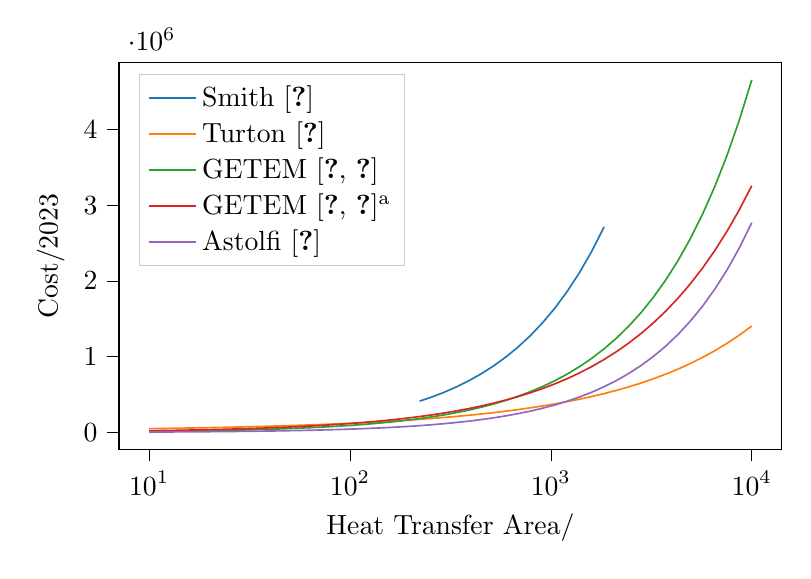
\begin{tikzpicture}

\definecolor{crimson2143940}{RGB}{214,39,40}
\definecolor{darkgray176}{RGB}{176,176,176}
\definecolor{darkorange25512714}{RGB}{255,127,14}
\definecolor{forestgreen4416044}{RGB}{44,160,44}
\definecolor{lightgray204}{RGB}{204,204,204}
\definecolor{mediumpurple148103189}{RGB}{148,103,189}
\definecolor{steelblue31119180}{RGB}{31,119,180}

\begin{axis}[
legend cell align={left},
legend style={fill opacity=0.8, draw opacity=1, text opacity=1, draw=lightgray204, at={(0.03, 0.97)}, anchor=north west},
log basis x={10},
tick align=outside,
tick pos=left,
unbounded coords=jump,
x grid style={darkgray176},
xlabel={Heat Transfer Area/\unit{\square\m}},
xmin=7.07945784384138, xmax=14125.3754462276,
xmode=log,
xtick style={color=black},
xtick={0.1,1,10,100,1000,10000,100000,1000000},
xticklabels={
  \(\displaystyle {10^{-1}}\),
  \(\displaystyle {10^{0}}\),
  \(\displaystyle {10^{1}}\),
  \(\displaystyle {10^{2}}\),
  \(\displaystyle {10^{3}}\),
  \(\displaystyle {10^{4}}\),
  \(\displaystyle {10^{5}}\),
  \(\displaystyle {10^{6}}\)
},
y grid style={darkgray176},
ylabel={Cost/\unit{\USD}2023},
ymin=-226908.054031314, ymax=4886629.18104146,
ytick style={color=black},
ytick={-1000000,0,1000000,2000000,3000000,4000000,5000000},
yticklabels={\ensuremath{-}1,0,1,2,3,4,5}, 
width=10cm, height=6.5cm
]
\addplot [semithick, steelblue31119180]
table {%
10 nan
11.5139539932645 nan
13.2571136559011 nan
15.2641796717523 nan
17.5751062485479 nan
20.2358964772516 nan
23.2995181051537 nan
26.8269579527973 nan
30.8884359647748 nan
35.5648030622313 nan
40.9491506238043 nan
47.1486636345739 nan
54.2867543932386 nan
62.5055192527397 nan
71.9685673001152 nan
82.8642772854684 nan
95.4095476349994 nan
109.854114198756 nan
126.48552168553 nan
145.634847750124 nan
167.683293681101 nan
193.069772888325 nan
222.29964825262 413491.732182502
255.954792269954 468766.563132901
294.705170255181 531430.434053867
339.322177189533 602471.098516923
390.693993705462 683008.351214217
449.843266896944 774311.678978008
517.947467923121 877820.271356679
596.362331659464 995165.706168561
686.6488450043 1128197.66761978
790.60432109077 1279013.10237386
910.298177991522 1449989.27315218
1048.11313415469 1643821.23088043
1206.79264063933 1863564.29604404
1389.49549437314 2112682.21887488
1599.85871960606 2395101.77750509
1842.06996932672 2715274.67470383
2120.95088792019 nan
2442.05309454865 nan
2811.76869797423 nan
3237.45754281764 nan
3727.59372031494 nan
4291.93426012878 nan
4941.71336132383 nan
5689.86602901829 nan
6551.28556859551 nan
7543.12006335462 nan
8685.11373751352 nan
10000 nan
};
\addlegendentry{Smith \cite{Smith2005}}
\addplot [semithick, darkorange25512714]
table {%
10 50105.271274881
11.5139539932645 52539.7597458259
13.2571136559011 55139.8197379762
15.2641796717523 57918.2186644687
17.5751062485479 60888.8322679748
20.2358964772516 64066.7493232015
23.2995181051537 67468.3870032167
26.8269579527973 71111.6180663199
30.8884359647748 75015.9111529455
35.5648030622313 79202.4856308801
40.9491506238043 83694.4825939213
47.1486636345739 88517.1538062772
54.2867543932386 93698.0705951317
62.5055192527397 99267.3549297904
71.9685673001152 105257.935191012
82.8642772854684 111705.829432321
95.4095476349994 118650.459270554
109.854114198756 126134.997920492
126.48552168553 134206.756313709
145.634847750124 142917.611721012
167.683293681101 152324.483838215
193.069772888325 162489.863904581
222.29964825262 173482.403111413
255.954792269954 185377.567335483
294.705170255181 198258.366110264
339.322177189533 212216.164741079
390.693993705462 227351.589593884
449.843266896944 243775.537859313
517.947467923121 261610.30453438
596.362331659464 280990.840996982
686.6488450043 302066.161400019
790.60432109077 325000.915212809
910.298177991522 349977.146622755
1048.11313415469 377196.264219804
1206.79264063933 406881.247466034
1389.49549437314 439279.119955582
1599.85871960606 474663.7234562
1842.06996932672 513338.831262683
2120.95088792019 555641.644563793
2442.05309454865 601946.721419867
2811.76869797423 652670.39467333
3237.45754281764 708275.742790389
3727.59372031494 769278.186398683
4291.93426012878 836251.793303931
4941.71336132383 909836.386223963
5689.86602901829 990745.560585313
6551.28556859551 1079775.7347329
7543.12006335462 1177816.37209255
8685.11373751352 1285861.53452943
10000 1405022.94874441
};
\addlegendentry{Turton \cite{Turton2012}}
\addplot [semithick, forestgreen4416044]
table {%
10 13117.3056360972
11.5139539932645 14787.1832243837
13.2571136559011 16669.6419049479
15.2641796717523 18791.7439733202
17.5751062485479 21183.9968472269
20.2358964772516 23880.7916423538
23.2995181051537 26920.8975802963
26.8269579527973 30348.0193363209
30.8884359647748 34211.4253393914
35.5648030622313 38566.6560569234
40.9491506238043 43476.322446596
47.1486636345739 49011.0060537921
54.2867543932386 55250.2736945019
62.5055192527397 62283.8213108091
71.9685673001152 70212.7634430674
82.8642772854684 79151.0868562683
95.4095476349994 89227.2892179849
109.854114198756 100586.226385588
126.48552168553 113391.194859402
145.634847750124 127826.279339226
167.683293681101 144098.999132781
193.069772888325 162443.291460937
222.29964825262 183122.874547851
255.954792269954 206435.03884389
294.705170255181 232714.920884134
339.322177189533 262340.321223583
390.693993705462 295737.135711888
449.843266896944 333385.478187825
517.947467923121 375826.582613571
596.362331659464 423670.58387414
686.6488450043 477605.289099029
790.60432109077 538406.065602919
910.298177991522 606946.987594833
1048.11313415469 684213.401901252
1206.79264063933 771316.093348496
1389.49549437314 869507.253446414
1599.85871960606 980198.481939792
1842.06996932672 1104981.08001843
2120.95088792019 1245648.92692181
2442.05309454865 1404224.26881334
2811.76869797423 1582986.79066589
3237.45754281764 1784506.38909716
3727.59372031494 2011680.1172984
4291.93426012878 2267773.83317813
4941.71336132383 2556469.14945601
5689.86602901829 2881916.36066337
6551.28556859551 3248794.10793067
7543.12006335462 3662376.63930521
8685.11373751352 4128609.63253593
10000 4654195.67035633
};
\addlegendentry{GETEM \cite{GETEM2016, Adams2021}}
\addplot [semithick, crimson2143940]
table {%
10 22537.3796240069
11.5139539932645 24945.0887116052
13.2571136559011 27610.0177221588
15.2641796717523 30559.6459259442
17.5751062485479 33824.3882534553
20.2358964772516 37437.9089173015
23.2995181051537 41437.468538902
26.8269579527973 45864.3083593533
30.8884359647748 50764.0754962388
35.5648030622313 56187.2936313951
40.9491506238043 62189.8839831038
47.1486636345739 68833.7419346866
54.2867543932386 76187.3752653777
62.5055192527397 84326.6105645564
71.9685673001152 93335.3751134912
82.8642772854684 103306.562296928
95.4095476349994 114342.989468164
109.854114198756 126558.458144584
126.48552168553 140078.927465806
145.634847750124 155043.813014487
167.683293681101 171607.424392503
193.069772888325 189940.556376003
222.29964825262 210232.250056435
255.954792269954 232691.742127462
294.705170255181 257550.622417723
339.322177189533 285065.221916734
390.693993705462 315519.25591792
449.843266896944 349226.749533397
517.947467923121 386535.275746812
596.362331659464 427829.539393219
686.6488450043 473535.344022021
790.60432109077 524123.982547074
910.298177991522 580117.096957879
1048.11313415469 642092.057202537
1206.79264063933 710687.914706505
1389.49549437314 786611.991916545
1599.85871960606 870647.175817595
1842.06996932672 963659.990629252
2120.95088792019 1066609.53292304
2442.05309454865 1180557.36129445
2811.76869797423 1306678.44256656
3237.45754281764 1446273.26739637
3727.59372031494 1600781.26021339
4291.93426012878 1771795.6217662
4941.71336132383 1961079.75732511
5689.86602901829 2170585.45993958
6551.28556859551 2402473.03624585
7543.12006335462 2659133.58235109
8685.11373751352 2943213.63949067
10000 3257642.48369385
};
\addlegendentry{GETEM \cite{GETEM2016, Adams2021}\textsuperscript{a}}
\addplot [semithick, mediumpurple148103189]
table {%
10 5525.45665381231
11.5139539932645 6272.92676267981
13.2571136559011 7121.51277900176
15.2641796717523 8084.89341262759
17.5751062485479 9178.5977954408
20.2358964772516 10420.2558018746
23.2995181051537 11829.8822321681
26.8269579527973 13430.1994392296
30.8884359647748 15247.0035996653
35.5648030622313 17309.5805330454
40.9491506238043 19651.177772173
47.1486636345739 22309.5404938508
54.2867543932386 25327.5199490361
62.5055192527397 28753.7641999231
71.9685673001152 32643.5022982282
82.8642772854684 37059.4345451744
95.4095476349994 42072.7431836446
109.854114198756 47764.2398142689
126.48552168553 54225.6680311226
145.634847750124 61561.1822747592
167.683293681101 69889.0267408231
193.069772888325 79343.4414072676
222.29964825262 90076.8259042203
255.954792269954 102262.19610681
294.705170255181 116095.973049798
339.322177189533 131801.149119678
390.693993705462 149630.882561415
449.843266896944 169872.578241166
517.947467923121 192852.520444481
596.362331659464 218941.132387993
686.6488450043 248558.947224839
790.60432109077 282183.386792916
910.298177991522 320356.457375449
1048.11313415469 363693.486524998
1206.79264063933 412893.041783418
1389.49549437314 468748.191181712
1599.85871960606 532159.28703246
1842.06996932672 604148.479082055
2120.95088792019 685876.190966289
2442.05309454865 778659.825560089
2811.76869797423 883995.000740693
3237.45754281764 1003579.65787235
3727.59372031494 1139341.43162719
4291.93426012878 1293468.72232778
4941.71336132383 1468445.97167929
5689.86602901829 1667093.71051547
6551.28556859551 1892614.02410468
7543.12006335462 2148642.16788998
8685.11373751352 2439305.16567894
10000 2769288.3348516
};
\addlegendentry{Astolfi \cite{Astolfi2014B}}
\end{axis}

\end{tikzpicture}
